\documentclass[12pt,fleqn]{article}\usepackage{../common}
\begin{document}
Minimum Kapsamli Agac (Minimum Spanning Tree -MST-)

MST algorithmasi kenar agirliklarina (weights) sahip olan bir cizit (graph)
yapisi icinde minimal ve kapsayan agaci (MST) bulan algoritmaya verilen
isimdir. Mesela alttaki cizit icinde

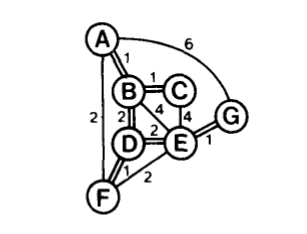
\includegraphics[height=4cm]{minspan_0.png}

MST oyle bir baglanti yapisidir ki bastan sona, herhangi bir noktadan
(node) bir digerine gecis yapilabilsin, ve bu tum yollarin toplami en
minimal olsun. Dikkat, herhangi bir noktadan digerine giden yol en az olsun
demiyoruz, bu durumda problem en kisa yol (shortest path) problemi
olurdu, ki bu problemi {\em Dinamik Programlama} yazisinda gorduk. Burada
gorecegimiz kapsayan agacin {\em toplaminin} minimal olmasidir. 

Kapsayan agac (spanning tree) kavramini tanimlamak gerekirse, bir cizitin
kapsayan agaci orijinal cizitin tum noktalarina sahip olmalidir, agac
icinde hicbir dongu (cycle) olmamalidir. Dongu derken bir noktadan digerine
atlaya atlaya giderken bizi donup tekrar ayni yere getirebilecek turden
``kapali devre'' tur bir donguden bahsediyoruz - bu mumkun
olmamalidir. Ayrica cizit baglantili olmalidir, yani bir kismi diger
kismindan kopuk bir cizit uzerinde MST bulunamaz. 

Minimum kapsayici agac ise bu tur pek cok alternatif agaclarin icinde en az
agirlikli olanidir. Not, bir cizitin MST cozumu tekil (unique) olmayabilir,
ayni agirlikta birden fazla degisik agac mumkundur. Mesela ustteki cizit
icin mumkun MST'ler altta goruluyor,

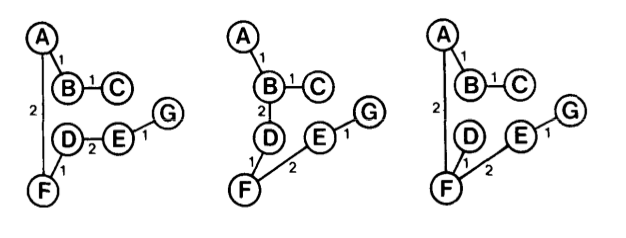
\includegraphics[height=4cm]{minspan_1.png}

Kontrol edilebilir, ustteki her agacin kenar toplami 8'dir. Bu agaclarin
her biri bir MST olarak kabul edilebilir.

Uygulama baglaminda MST bulma algoritmasinin ne kadar kullanisli olacagi
goruluyor herhalde; mesela elektrik hatlari, telefon iletisim hatlari
tasarlarken MST kullanilabilir, toplam baglantisi en az olan bir ag yapisi
her iki durumda da kullanisli olur. Biyolojik, kimyasal aglarin analizinde
bile MST kullanilmaktadir.

Agaclarin Ozellikleri (Properties of Trees)

Baslamadan once bir agaci agac yapan iki onemli ozelligi belirtelim

1) Tanim itibariyle agac olan bir seye, arasinda baglanti olmayan iki
noktayi birlestiren bir kenar koyarsak bu agacta bir dongu yaratmis
oluruz.

2) Elde olan bir agacin herhangi bir kenarini cikartirsak bu agaci
``kopartmis'' oluruz, birbiriyle baglantisiz iki alt-agac ortaya cikar.

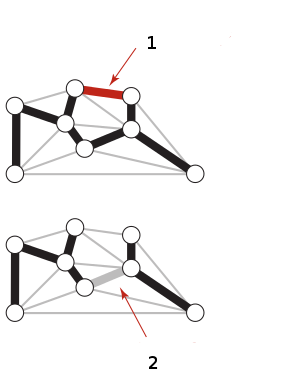
\includegraphics[height=8cm]{graph_prop.png}

Resimde her iki durumu goruyoruz. Bu iki ozellik cok onemli, cunku onlari
MST'lerin cok temel ozelliklerini ispatlamak icin kullanacagiz. Ondan once
bazi tanimlar,

Tanim

Kesik (cut): Bir cizit uzerindeki yapilan kesik, o ciziti birbiriyle
alakasiz, baglantisiz iki parcaya / kumeye boler. {\em Not}: Bir kesik
birden fazla kenarin uzerinden gecebilir / kapsayabilir, cunku bir ciziti
tamamen ikiye ayirmaktan bahsediyoruz. Bir agactan bahsediyor olsaydik,
yukarida belirttigimiz gibi, tek bir kenari kesmek yeterli olurdu.

Birlestiren kenar (crossing edge): birbirinden baglantisiz iki kumedeki
herhangi bir noktayi diger kumedeki herhangi bir diger noktayla birlestiren
bir kenardir.

Onerme (Proposition)

Herhangi bir ciziti alalim, ve bu cizitteki bir kesik icindeki (yani
kopardigi tum kenarlar) icindeki minimum birlestiren kenara bakalim. Bu
kenar o cizitin MST'sinde {\em kesinlikle} olmalidir.

Ispat

Bu ispat tersini yanlislama (proof by contradiction) yontemini
kullanacak. Diyelim ki bir kesik var, ve o kesikteki $e$ minimum
birlestiren kenar. Bu cizitin MST'si $T$ olsun. Simdi $e$'nin $T$'nin
icinde olmadigi durumu dusunelim (yani onermenin dediginin tersi), ve
diyelim ki simdi $e$'yi alip $T$'ye ekliyoruz. Yeni bir cizit ortaya
cikardi, fakat daha once dedigimiz gibi, $T$'ye bir kenar eklemek ona ayni
zamanda bir dongu eklemek demektir, ki bu dongunun icinde en az bir diger
kenar $f$ olacaktir (cunku $e$ MST'de olmadigina gore orada baska bir sey
var), ki bu $f$, $e$'den buyuktur. Fakat o zaman $f$'yi kesip onun yerine
daha az agirlikta olan $e$'yi ekleyince MST'yi, hem de daha az agirlikla
elde etmis olmaz miydik? Evet. Demek ki $e$'nin MST icinde olmamasi
imkansizdir cunku MST tanim itibariyle en minimal agirliga sahip olmalidir.

Alttaki resimde gri ve beyaz ile gosterilen ayri kumelerdeki noktalari bir
kesik ile ayrilmislar ve bu kumelerin arasindaki birlestiren kenarlar
kirmizi ile gosteriliyor. Burada $e$ ile gosterilen kenar MST icinde
olmalidir. 

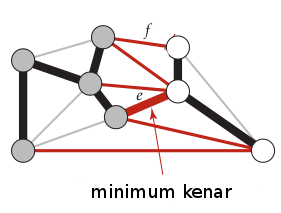
\includegraphics[height=5cm]{cross_edge.png}

Ustteki kavramlar Kruskal'in MST bulan algoritmasinin temelini
olusturmaktadir (bu algoritmaya kisaca Kruskal diyecegiz). Kruskal (ilk
basta) birbirinden bagimsiz agaclari yavas yavas yaratir, onlari
buyutur. Ayni anda surekli o agaclari minimal bir kenar ile birlestirip
onlari daha buyuk bir agac yapma firsatina bakar. 

Ufak ufak agaclar ustteki durumda gri ve beyaz noktalari kapsayan agaclar
gibi gorulebilir, bunlar cizitin farkli bolgelerinde ayri ayri
buyurler. Eger bu ayri ayri bolgelerde, onlara ait MST'ler
olusturabilmissek, Onlari minimal sekilde birlestirmek (ustte $e$ ile) bize
daha buyuk bir MST saglar. 

Kruskal kenarlari teker teker isler, once onlari agirliklarina gore
siralar, ve en kucuk kenarlari once alir. Bu yuzden agaclari baglanayan
``birlestiren kenarin'' minimal kalmasi, ve once alinmasi da saglanir.

Birlesim-Bulus (Union-Find)

Kruskal'in kodlama baglaminda onemli bir puf noktasi, sirayla bakilan bir
kenarin mevcut alt-agaclardan birine eklenme durumunda dongu olusturup
olusturmadigini hizli bir sekilde anlayabilmesidir. Bunun icin su diger
soruyu cevaplamak yeterlidir: bir kenara baktigimizda, bu kenarin iki
ucundaki iki noktayi aliriz, ve bu iki noktanin herhangi bir alt-agac
icinde, yani ayni alt-agac icinde, olup olmadigina bakariz (hatirlarsak pek
cok alt-agac olabiliyor). Eger bu iki nokta herhangi bir alt-agac icinde
bulunursa, bu kenari cope atabiliriz, cunku bu noktalar baska bir sekilde
bir alt-MST olusturmustur, ve bu alt-MST optimaldir (bkz ustteki ispat).

``Iki noktanin ayni alt agac icinde olup olmadigini anlamak'' ise su
alt-agaclarin surekli bir ``temsili noktaya'' isaret etmesiyle
halledilebilir (bu isaret, kenarlardan farkli). Eger iki nokta, ayni,
temsili noktaya isaret ediyorsa, onlar ayni agac icindedir, vep dolayli
olarak bu demektir ki bu noktalar bir sekilde ``baglanmistirlar'' cunku her
alt-agac ayni zamanda ufak bir MST'dir. Bu durumda yeni kenari eklemek
tanim itibariyle bir dongu olusturur, ve gereksizdir. Eger noktalar farkli
agaclarda iseler, bu agaclari birlestirmek iki temsili noktadan birinin bir
digerine isaret etmesiyle halolabilir. Evet birlestirme sonrasi bazi uyeler
yeni temsili noktaya isaret etmiyor olabilirler, bu durum, noktadan noktaya
atlanip temsili noktaya erismek ile halolur. Bu arada, arama sirasinda,
yeni temsili noktaya olan isaretler degistirilir, ki bu ``duzeltme'' islemi
yol sikistirma (path compression) olarak aniliyor.

Alttaki kod tum bu numaralari kullaniyor. Ornek olarak yazinin basinda
verilen ciziti kodladik ve MST'sini bulduk. Cizit formati iki yonlu
kenar bilgisi gerektirmez, iki nokta arasindaki gecisi bir kere belirtmek
yeterlidir. 

\begin{minted}[fontsize=\footnotesize]{python}
G1 = {
  'a': {'b':1, 'f':2, 'g': 6},
  'b': {'c':1},
  'c': set(),
  'd': {'f':1, 'e':2},
  'e': {'g':1},
  'f': set(),
  'g': set()
}
\end{minted}


\begin{minted}[fontsize=\footnotesize]{python}
def find(C, u):
    if C[u] != u:
        C[u] = find(C, C[u])                    # Path compression
    return C[u]

def union(C, R, u, v):
    u, v = find(C, u), find(C, v)
    if R[u] > R[v]:                             # Union by rank
        C[v] = u
    else:
        C[u] = v
    if R[u] == R[v]:                            # A tie: Move v up a level
        R[v] += 1

def kruskal(G):
    E = [(G[u][v],u,v) for u in G for v in G[u]]
    T = set()
    C, R = {u:u for u in G}, {u:0 for u in G}   # Comp. reps and ranks
    print list(sorted(E))
    for _, u, v in sorted(E):
        if find(C, u) != find(C, v):
            T.add((u, v))
            print (u, v)
            union(C, R, u, v)
    return T

mst = list(kruskal(G1))
print 'MST', mst
\end{minted}

\begin{verbatim}
[(1, 'a', 'b'), (1, 'b', 'c'), (1, 'd', 'f'), (1, 'e', 'g'), (2, 'a', 'f'), (2, 'd', 'e'), (6, 'a', 'g')]
('a', 'b')
('b', 'c')
('d', 'f')
('e', 'g')
('a', 'f')
('d', 'e')
MST [('d', 'e'), ('e', 'g'), ('d', 'f'), ('b', 'c'), ('a', 'f'), ('a', 'b')]
\end{verbatim}

Bu isleyis (yine basta gosterdigimiz) alternatif MST'lerden birincisini
buldu (\verb!a-f! bagli, \verb!e-f! bagli degil). Guzel! Kruskal'in isleyis
hizi $O(E \log E)$ seviyesindedir, $E$ kenar sayisidir. Bu cok iyi bir
performanstir, bu performansin mesela $O(N^2)$'den farkini gostermek icin
alttaki hesaba bakalim, eger 100,000 tane kenar olsaydi,

\begin{minted}[fontsize=\footnotesize]{python}
e = 100 * 1000
print 'n^2', e**2
print 'log', np.log(e)
print 'kruskal', e*np.log(e)
\end{minted}

\begin{verbatim}
n^2 10000000000
log 11.512925465
kruskal 1151292.5465
\end{verbatim}

Kruskal 1 milyon kusur operasyona orantili bir sonuc verirdi, kiyasla
$O(N^2)$ 10 milyar operasyon ortaya cikartiyor! 

Bir diger ornek: Altta MST'nin adim adim olusturulmasini da
gorecegiz. Kirmizi ile isaretlenen kenar o adimda secilen kenari
gosteriyor, siyah olanlar mevcut MST(lerde) olan kenarlari.


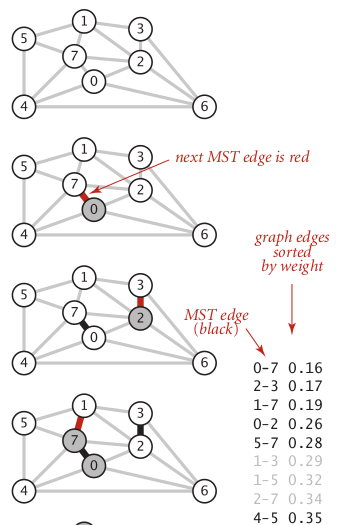
\includegraphics[height=9cm]{sedge_krus_1.png}

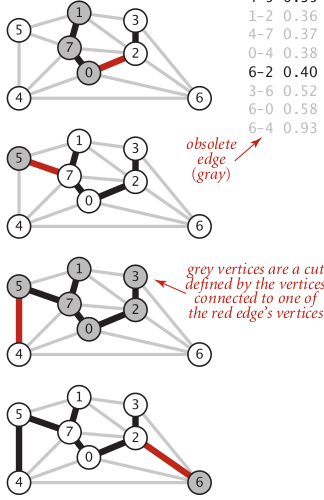
\includegraphics[height=9cm]{sedge_krus_2.png}


\begin{minted}[fontsize=\footnotesize]{python}
G2 = {
  0: {7: 0.16, 4: 0.38, 2: 0.26, 6: 0.58},
  1: {5: 0.32, 2: 0.36, 3: 0.29, 7: 0.19},
  2: {3: 0.17, 6: 0.40, 7: 0.34},
  3: {6: 0.52},
  4: {5: 0.35, 7: 0.37, 6: 0.93},
  5: {7: 0.28},
  6: set(),
  7: set()
} 

mst = list(kruskal(G2))
print 'MST', mst
\end{minted}

\begin{verbatim}
[(0.16, 0, 7), (0.17, 2, 3), (0.19, 1, 7), (0.26, 0, 2), (0.28, 5, 7), (0.29, 1, 3), (0.32, 1, 5), (0.34, 2, 7), (0.35, 4, 5), (0.36, 1, 2), (0.37, 4, 7), (0.38, 0, 4), (0.4, 2, 6), (0.52, 3, 6), (0.58, 0, 6), (0.93, 4, 6)]
(0, 7)
(2, 3)
(1, 7)
(0, 2)
(5, 7)
(4, 5)
(2, 6)
MST [(2, 6), (4, 5), (5, 7), (0, 7), (2, 3), (1, 7), (0, 2)]
\end{verbatim}

Sekilde \verb!5-7!'yi birbirine baglayan 6. adim sonrasi \verb!1-3!'un
cozume dahil edilmedigine dikkat edelim. Bu noktada 1 ve 3 dugumleri artik
ayni agac icindedirler, ve bu kenari eklemek bir dongu olusturacaktir. 

Kruskal algoritmasi, ve ona benzer Prim, ya da ``bir sonraki adimda hep en
yakini isleyen'' algoritmalar acgozlu (greedy) algoritmalar olarak
bilinirler. Mesela {\em Dinamik Programlama} yazisinda gordugumuz uzere,
acgozlu yontem en kisa yolu vermeyebiliyordu. MST durumunda acgozluluk
faydalidir, acgozlulugun faydali oldugu mutlu orneklerden biridir diyelim! 

Not: Bazilarina tanidik gelebilecek bilgisayar bilimin demirbas
problemlerinden Seyahat Eden Satis Gorevlisi (Traveling Salesman Problemi
-TSP-) NP-Tam olarak bilinir. MST, ki cok hizli isleyen bir algoritma,
yaklasiksal olarak TSP'yi cozmekte kullanilabilmektedir. 

Sedgewick, R. {\em Algorithms}, sf. 409

Sedgewick, R. {\em Algorithms, 4rd Edition}, sf. 624

Heatland, {\em Python Algorithms}

\end{document}
